\chapter{Foundations}
\label{sec:foundations}

This chapter introduces the foundations for working with story diagrams.
Since story diagrams are based on graphs and corresponding graph transformations,
we introduce the basics of graph transformations in Section \ref{sec:foundations:simpleGTS}.
Story diagrams are built on an extension of this simple graph model which is called typed attributed graph transformations (cf.\ Section \ref{sec:foundations:typedAttrGTS}).
These are based on so-called type graphs that allow to distinguish different types of nodes and edges.
Based on typed attributed graph transformations, we will introduce basic concepts of model transformations in Section~\ref{sec:modelTransformation}.
Section~ \ref{sec:typeGraph} presents a type graph which we use in the examples in this document.

\section{Graphs and Graph Transformations}
\label{sec:foundations:simpleGTS}

Graphs consist of nodes and edges where an edge always connects two nodes. Nodes are used to represent objects and edges denote relationships between these objects. In the course of this document, we assume edges to be directed, i.e., they have a source node and a target node. In the most simple case, neither nodes nor edges have a predefined semantics~\cite{Roz97}.

\begin{figure}[htbp]
  \centering
  
\includegraphics[scale=1.5]{figures/SimpleGraph}
  \caption{Simple Graph}
  \label{fig:simpleGraph}
\end{figure}

Figure~\ref{fig:simpleGraph} shows an example of a simple graph with three nodes and four directed edges. The nodes are visualized as circles, the edges are visualized as arrows. An edge may have the same node as a source and target node. Such an edge is called a \emph{self-edge}. 

\emph{Graph transformation rules} specify allowed modifications of graphs. They consist of a left-hand side (LHS), a right-hand side (RHS), and a so-called rule morphism. Both, the LHS and the RHS are graphs while the rule morphism specifies which nodes of the LHS and RHS are considered to be the same. This information is required for the application of a graph transformation rule to a graph.

\begin{figure}[htbp]
  \centering
  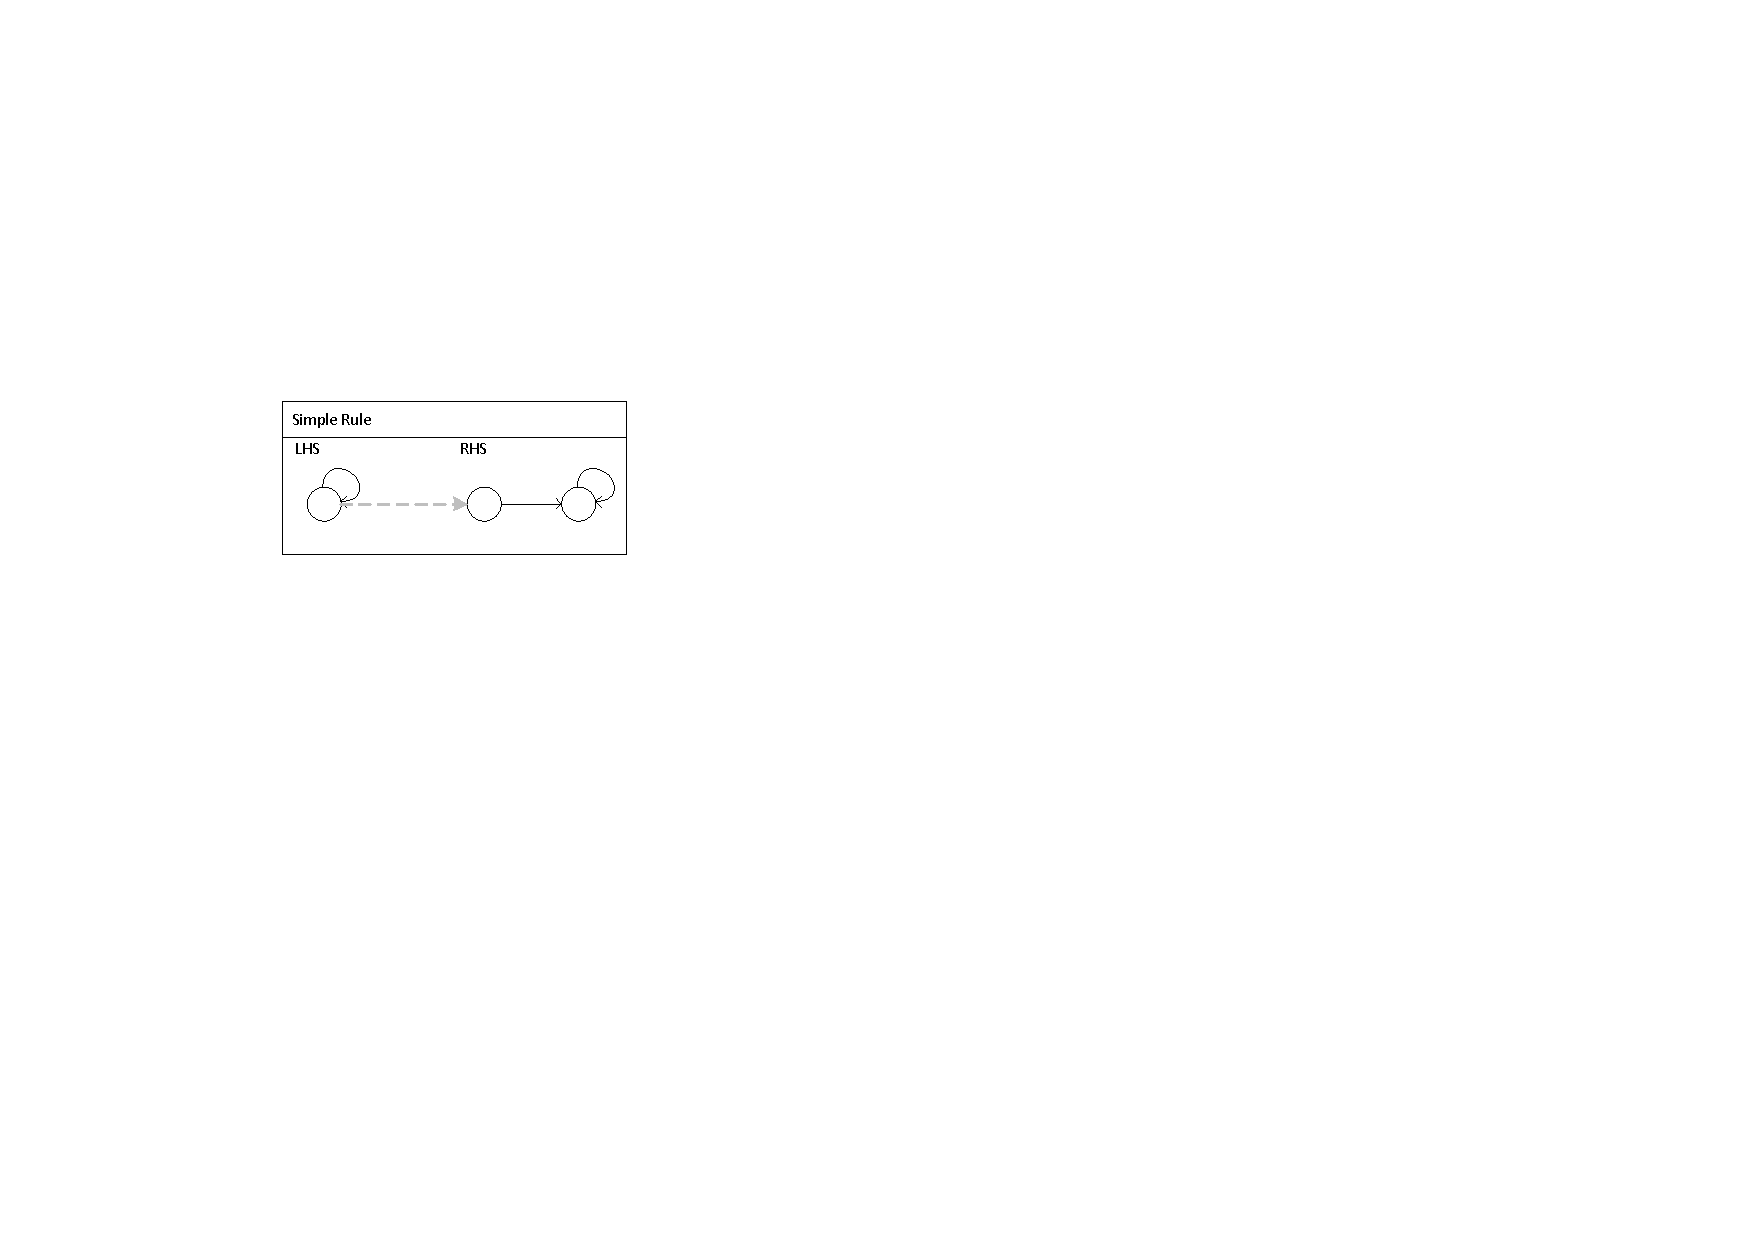
\includegraphics[scale=1.5]{figures/SimpleGTRule}
  \caption{Simple Graph Transformation Rule}
  \label{fig:simpleGTRule}
\end{figure}

Figure~\ref{fig:simpleGTRule} shows an example of a graph transformation rule. The LHS contains only one node with a self-edge. The RHS contains two nodes connected by an edge where the right node of the RHS has a self-edge as well. The rule morphism is visualized by the gray, dotted arrow. It specifies that the node of the LHS and the left node of the RHS are considered to be the same.

The application of a graph transformation rule to a graph is called a \emph{graph transformation}~\cite{EEPT06}. The graph on which the rule is to be applied is called the \emph{host graph}.
The application of a graph transformation rule to a graph is performed in three steps. In the first step, an occurrence of the LHS of the graph transformation rule in the host graph is searched. Such an occurrence is called a \emph{match} of the graph transformation rule. If a match has been found, the second step is executed in which all nodes and edges that occur in the LHS but not in the RHS are deleted from the host graph. In this step, the rule morphism is used to decide which nodes do not occur in the RHS. In the third step, all nodes and edges that occur in the RHS but not in the LHS are added to the host graph. After the application of the graph transformation rule, there exists a match of the RHS into the host graph.

\begin{figure}[htbp]
  \centering
  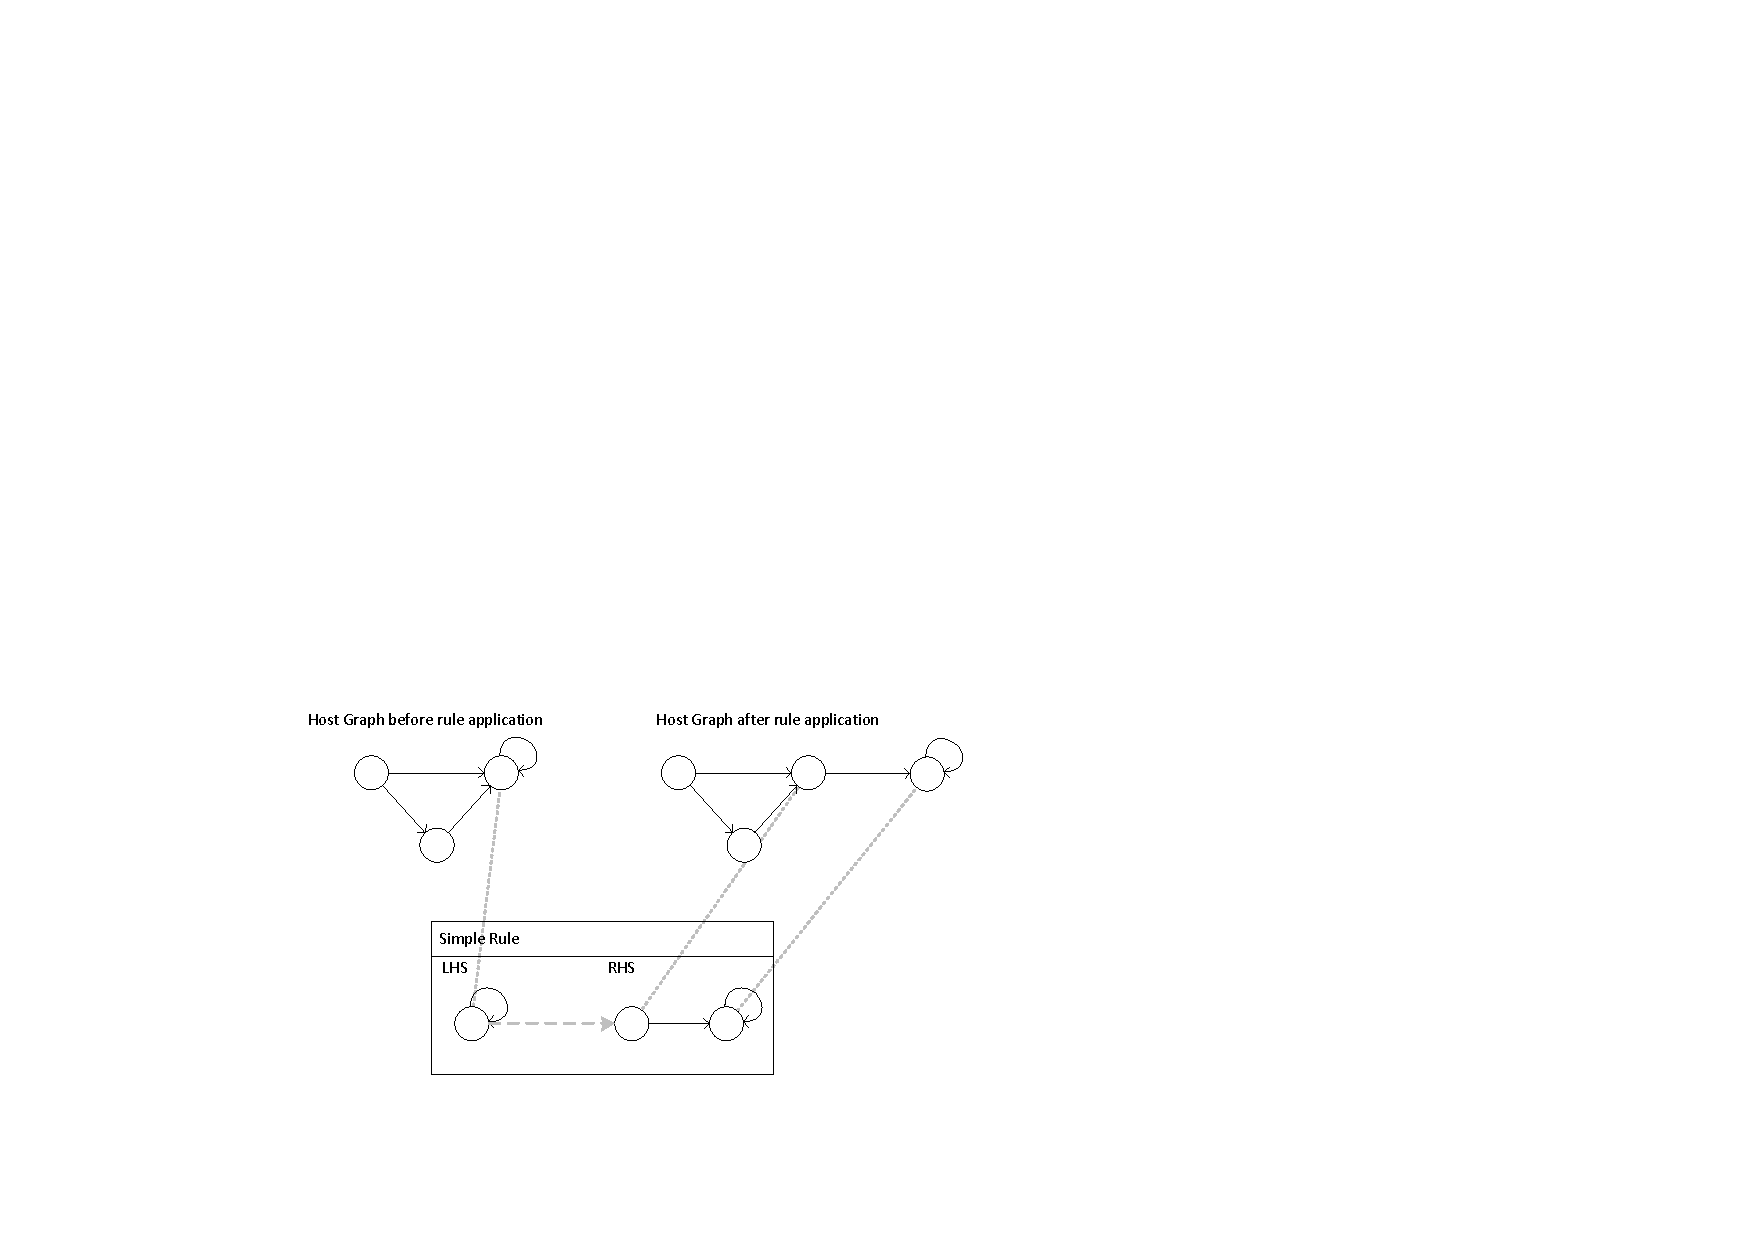
\includegraphics[width=\linewidth]{figures/GTApplication}
  \caption{Application of a Graph Transformation Rule}
  \label{fig:GTApplication}
\end{figure}

Figure~\ref{fig:GTApplication} shows an example of a graph transformation that applies the graph transformation rule of Figure \ref{fig:simpleGTRule} to the graph of Figure~\ref{fig:simpleGraph}. The matching of the LHS into the host graph is visualized by a gray, dotted line. Then, the graph transformation rule deletes the self-edge from this node. Afterwards, a new node with a self-edge is created and connected to the previously matched node by an edge. The match of the RHS into the host graph after the rule application is again shown by gray, dotted lines.

Formally, identifying a matching of a graph transformation rule in a host graph requires to identify a subgraph of the host graph which is isomorphic to the LHS. This is denoted as the \emph{subgraph isomorphism} problem which is known to be \emph{NP-complete}~\cite{Epp95}. 

In the field of algebraic graph transformations, the two most popular approaches for applying a graph transformation rule to a graph are the
\emph{double-pushout approach} \cite{Roz97} and the \emph{single-pushout
approach} \cite{Roz97}. The definition of story diagrams follows the
single-pushout approach. Besides the more theoretical differences, the two
approaches differ in the handling of two special situations that might occur
upon rule application.

The first situation is the following. Assume the left-hand side of a rule
consists of two nodes. The first node is to be deleted and the second one is
to be preserved. Both of these nodes may be matched to the same node in the host
graph. In this situation, it is not clear if the node in the host graph is to be
deleted or preserved. The double-pushout approach explicitly forbids the application of the rule in such
situations. The single-pushout approach allows such situations and gives
deletion priority over preservation.

The second situation deals with dangling edges. It occurs if a certain node is
to be deleted but some of its connected edges are to be preserved. The
transformation would lead to a non-valid graph in which the edges would no longer have
either a source or a target node. The double pushout approach does not allow
such situations and instead requires that connected edges are explicitly
deleted. The single-pushout approach allows such situations and implicitly
deletes edges if one of their source or target nodes is deleted.

In general, matches of graph transformation rules are homomorphisms of the LHS of the rule to the host graph.
That allows to match two nodes of the LHS to the same node of the host graph leading to the first situation mentioned above.
Such situations may be prevented by using isomorphisms for matching the LHS. Then, each node of the LHS must be matched to a unique node of the host graph.
Thus, using isomorphic matchings prevents the first situation when using single-pushouts.

In addition to LHS and RHS a graph transformation rule may specify negative application conditions (NAC,~\cite{Roz97}).
A NAC is an additional condition for a successful match.
If the subgraph specified by the NAC can be matched into the host graph, then the graph transformation rule must not be applied.

%In story diagrams, we use a graph transformation language called \emph{story patterns}.
%A story pattern is a graph transformation rule which is executed on a host graph by identifying a subgraph in the host graph
%that is similar to the one specified in the graph transformation rule
%and then removing and adding the specified nodes and edges.
%The identification of the subgraph for modification is called \emph{graph matching} and includes the \emph{subgraph isomorphism} problem.
%The subgraph isomorphism problem, in general, is \emph{NP-complete} \cite{Epp95}.
%To reduce the problem in the average case, the implemented graph matching approach based on story patterns
%uses a subgraph isomorphism for at least one node as input,
%i.e.\ at least one node in the left-hand side of a graph transformation rule (a story pattern) is already matched to a certain node in the host graph.


\section{Typed Attributed Graph Transformations}
\label{sec:foundations:typedAttrGTS}

Graphs and according graph transformations as introduced in Section \ref{sec:foundations:simpleGTS} are a very basic approach to modeling behavior.
When using graph transformations for modeling behavior for object-oriented software or as a foundation for defining the semantics of modeling languages,
it is necessary to distinguish different types of nodes and edges in a graph in order to give them semantics.

\begin{figure}[htb]
  \centering
  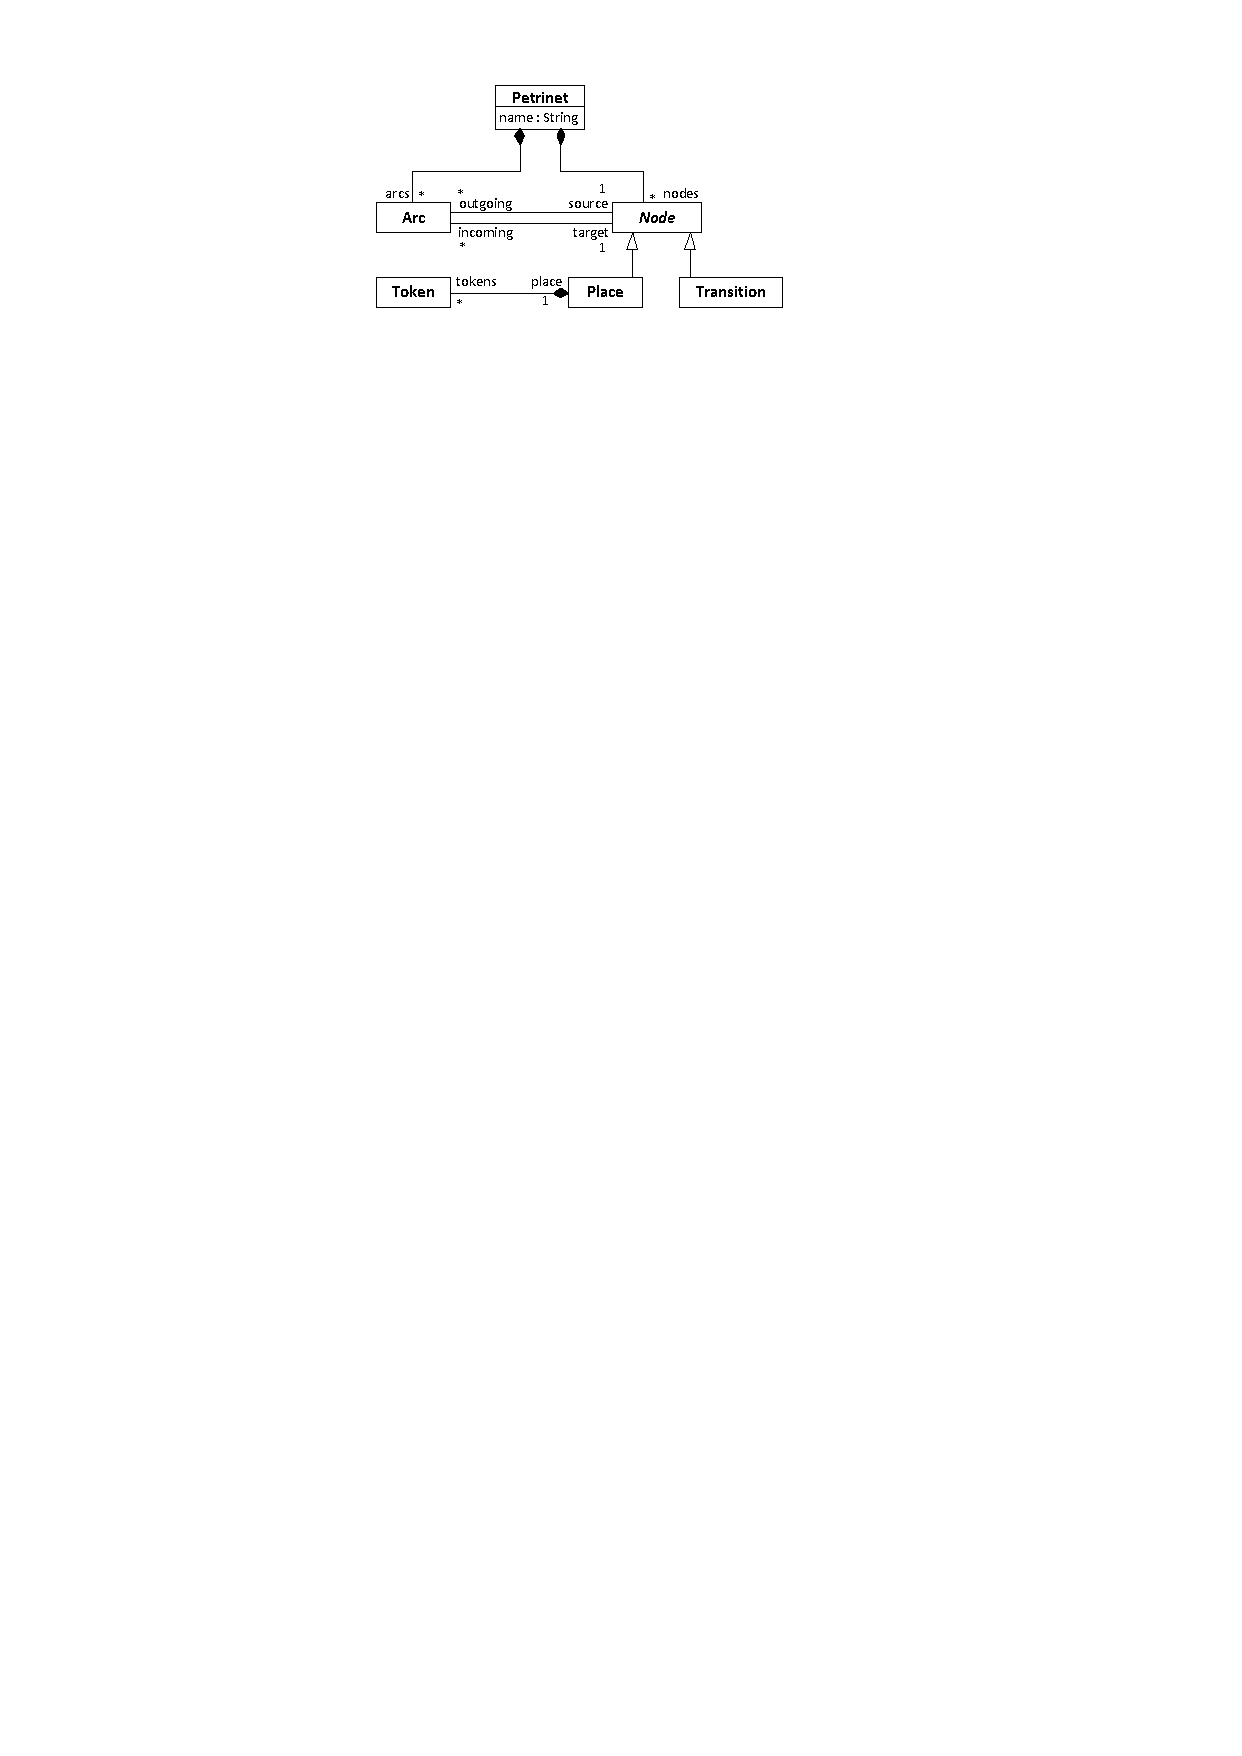
\includegraphics[scale=1]{figures/Petrinet}
  \caption{An Exemplary Type Graph -- Metamodel for Petrinets}
  \label{fig:PetrinetTypeGraph}
\end{figure}

Therefore, \emph{typed attributed graph transformations} \cite{EEPT06} have been defined.
Typed attributed graph transformations introduce a \emph{type graph} and node attributes.
The type graph defines different types of nodes and edges and it defines which types of edges are allowed to be used in combination with which types of nodes.
Additionally, nodes may carry attributes like, e.g., objects in an object-oriented programming language.
Moreover, the type graph specifies inheritance relations between types of objects, a concept which is also known from object-oriented programming languages. Thereby, a type graph specifies the structure of all possible graphs.

As an example, Figure~\ref{fig:PetrinetTypeGraph} shows a simple type graph for petrinets.
A \fe{Petrinet} consists of \fe{Nodes} and \fe{Arcs}.
An \fe{Arc} connects two nodes which it refers as \fe{source} and \fe{target}.
As usual, there exist two types of nodes: \fe{Places} and \fe{Transitions} where \fe{Places} may contain a number of \fe{Tokens}.

The type graphs can be created, e.g., by using an arbitrary metamodeling language.
Examples include Ecore~\cite{SBP+08}, MOF~\cite{MOF05}, and UML~\cite{UML23}.

The modifications of a typed attributed graph are specified by typed attributed graph transformation rules.
In these rules, all nodes and edges are typed over the type graph  and the matching needs to respect the types.

\begin{figure}[htb]
  \centering
  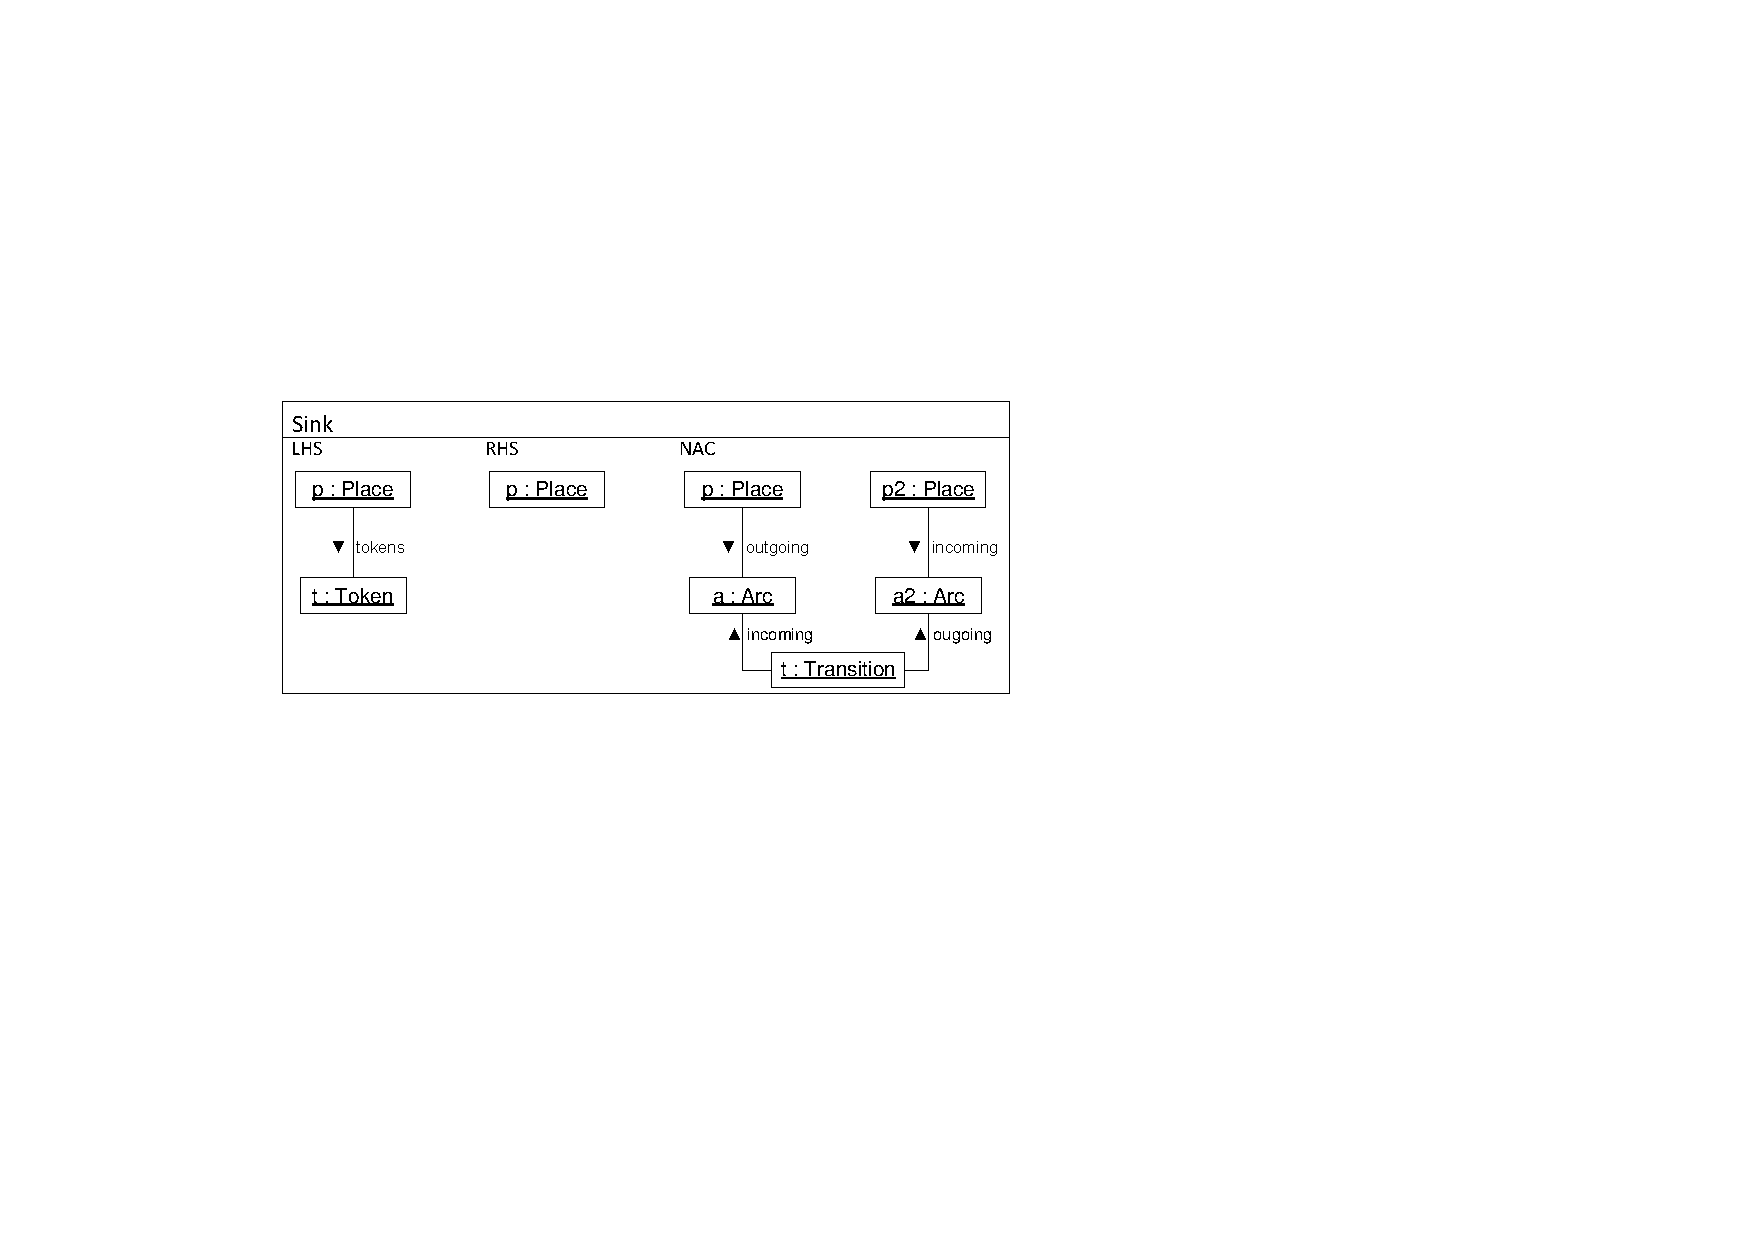
\includegraphics[scale=1]{figures/TypedGTRule}
  \caption{Typed Attributed Graph Transformation Rule}
  \label{fig:typedGTRule}
\end{figure}

Figure~\ref{fig:typedGTRule} shows an example of a typed attributed graph transformation rule using a concrete syntax as used by Ehrig et al.~\cite{EEPT06} that specifies the behavior for a sink.
In a petrinet, a sink is a transition which has no outgoing place.
Then, the transition consumes tokens without producing new tokens.
The rule matches a \fe{Place} with a \fe{Token} in its LHS.
Upon application, the \fe{Token} is deleted.
The rule, however, may only be applied if the place \fe{p} is connected to a sink which is ensured by the NAC.
The NAC specifies a subgraph where \fe{p} is connected to a \fe{Transition} which has an outgoing \fe{Arc} to a \fe{Place}.
If such subgraph can be matched, the rule is not applicable.
The rule morphisms is indirectly specified by the names of the nodes as proposed by Ehrig et al.~\cite{EEPT06}.


\section{Model Transformations}
\label{sec:modelTransformation}

A model transformation modifies or translates different kinds of models.
We use graph transformations to specify model transformations formally.
In the context of model transformations, the host graph of a graph transformation is called \emph{instance model}\footnote{Thomas K\"{u}hne calls it \emph{token model} \cite{Kue06}.} (or simply model).
Instance models are specified in a certain language, often a domain-specific language (DSL)\footnote{The language can be both, textual or graphical.}.
Thus, the type graph usually defines the \emph{abstract syntax} of the language used and is part of the corresponding \emph{metamodel} \cite{Kue06} for this language.
By replacing the type graph (the metamodel) we are able to specify transformations for models specified in various languages.

The type graph or the abstract syntax of the language used to describe the instance models
is, in our case, described by a set of classes and their relations which define all potential instance models.
These classes and relations constitute a so-called \emph{type model} (the actual type graph).
An instance model always contains \emph{objects} and \emph{links} (nodes and edges) that are instances of the classes and relations defined in the corresponding type model.

If a graph transformation transforms a model based on a given type graph into a model based on the same type graph (modification of the model),
the transformation is called \emph{endogenous} (also known as \emph{in-place} transformation).
Otherwise, i.e., the transformation transforms a model based on a given type graph into a model based on another type graph (translation),
the transformation is called \emph{exogenous} (also known as \emph{model-to-model} transformation).
In principle, story diagrams are endogenous graph transformations.
By combining the type graphs of the source model and the target model, story diagrams may also be used to specify exogenous graph transformations.

\section{The Type Graph in The Running Example}
\label{sec:typeGraph}

The type graph used in the examples in this report describes the structure of an abstract syntax tree for programming languages.
In particular, it is an updated and slightly simplified version of the generalized abstract syntax tree (GAST) metamodel developed in the QBench project~\cite{QBench}.
The GAST was developed to provide a unified syntax tree model for different programming languages like Java, C, and C++.
Figure~\ref{fig:gast-mm} shows an excerpt of that metamodel.
Some specialized subclasses have been omitted for clarity reasons.

\begin{figure}[htbp]
  \centering
  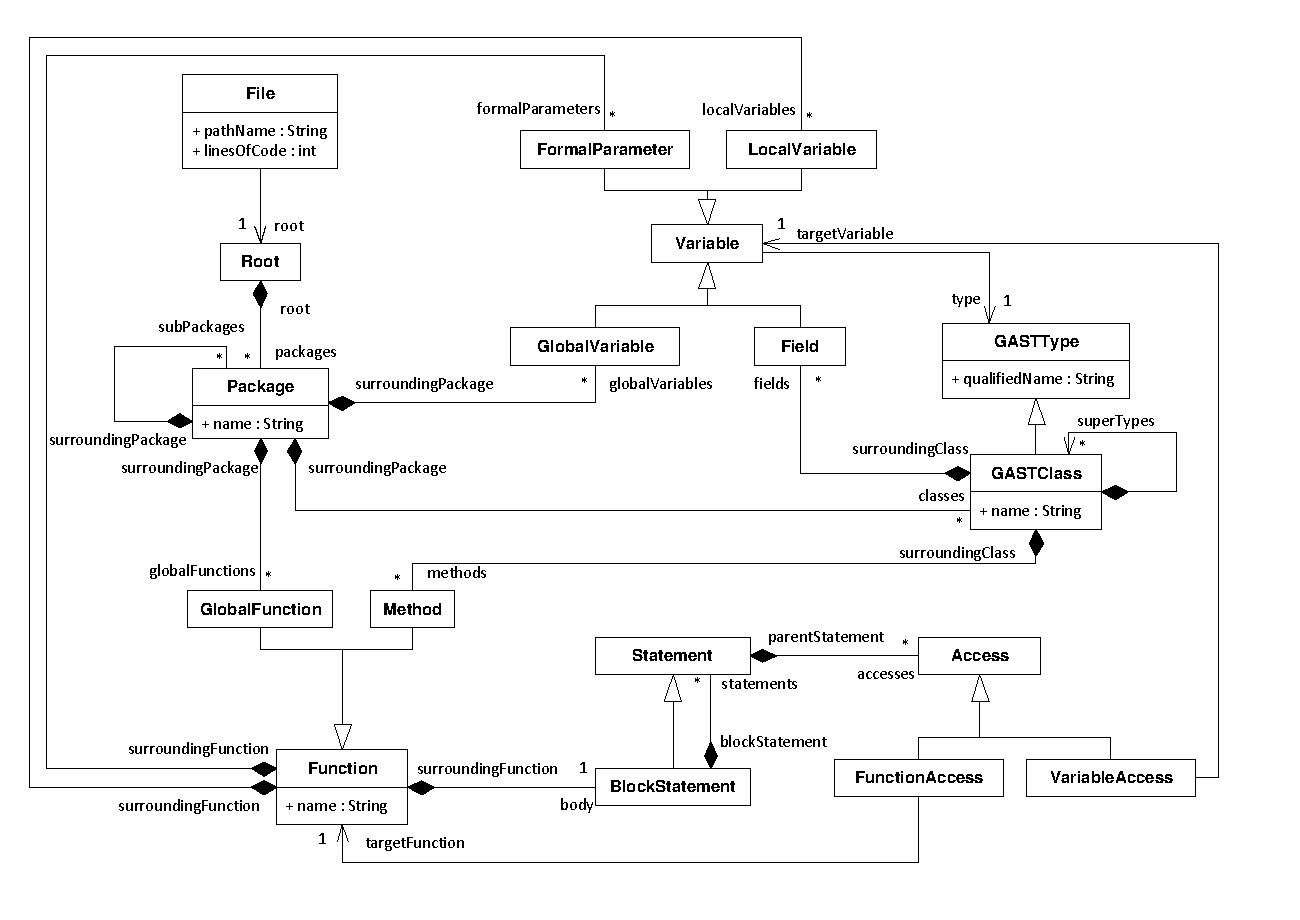
\includegraphics[width=\linewidth]{figures/gast-mm}
  \caption{Type Graph of a Generalized Abstract Syntax Tree (GAST) for Object-Oriented Programming Languages \cite{QBench}}
  \label{fig:gast-mm}
\end{figure}

The following description of the classes in the type graph is based on \cite{Tra11}.

\begin{description}
\item[Root] The \fe{Root} element is the central element of every GAST model. All other elements are reachable from the \fe{Root} node via composition relations.
\item[File] Elements of the GAST, e.g., classes and packages, can be assigned to files in the file system. A \fe{File} element holds references to those classes and packages and a String containing the path to the file.
\item[Package] Similar to packages in Java, the \fe{Package} element provides name spaces and visibilities. A \fe{Package} element can contain other packages, classes, global variables, and functions.
\item[GASTType] The \fe{GASTType} element represents data types like primitive data types and classes. The attribute \fe{qualifiedName} contains the unique, fully qualified name of the type.
\item[GASTClass] Classes are represented by the element \fe{GASTClass} in the GAST and are a sub type of the \fe{GASTType}. A \fe{GASTClass} holds references to its methods, attributes, and inner classes. A \fe{GASTClass} can be assigned to a \fe{Package}.
\item[Function] \fe{Function} is the super type for all executable operations. In addition to a name attribute, a \fe{Function} can have a number of local variables and formal parameters. The return type of a \fe{Function} is determined by its \fe{DeclarationTypeAccess}, a sub class of \fe{Access}. A \fe{Function} always contains a block statement which, in turn, can contain other statements.
\item[GlobalFunction] A \fe{GlobalFunction} element represents a globally accessible operation, i.e., an operation that does not belong to a class. It can be assigned to a name space defined by a package. For example, C functions are represented by \fe{GlobalFunctions}.
\item[Method] Functions that belong to a class are represented by \fe{Method} elements, a sub type of \fe{Function}.
\item[Variable] \fe{Variable} is a super type for all kinds of variables. A \fe{Variable} always has a name and a type.
\item[LocalVariable] \fe{LocalVariables} are variables that are contained in a \fe{Function}.
\item[FormalParameter] \fe{FormalParameters} are variables that represent the parameters of a \fe{Function}.
\item[GlobalVariable] \fe{GlobalVariables} are variables that are globally accessible within a given scope. The scope is determined by the package in which the \fe{GlobalVariable} is contained.
\item[Field] The \fe{Field} element represents class variables. Therefore it is contained in a \fe{GASTClass}.
\item[Statement] A \fe{Function} consists of a number of \fe{Statements}. There are multiple sub classes of \fe{Statement} which represent the different kinds of statements. Most of them are omitted here. A \fe{Statement} can contain a number of \fe{Accesses}.
\item[BlockStatement] The \fe{BlockStatement} is a special kind of statement which can contain other \fe{Statements}. It is the root element of all \fe{Statements} contained within a \fe{Function}.
\item[Access] An \fe{Access} represents the use of a \fe{Variable} or a \fe{Function}. It always belongs to a certain \fe{Statement}.
\item[FunctionAccess] A \fe{FunctionAccess} represents the use of a \fe{Function} in a \fe{Statement} and therefore references the accessed \fe{Funtion} element.
\item[VariableAccess] A \fe{VariableAccess} represents the use of a \fe{Variable} in a \fe{Statement} and therefore references the accessed \fe{Variable} element.
\end{description}
